\documentclass[12pt,a4paper]{article}
\usepackage[margin=0.9in]{geometry}
\usepackage[T1]{fontenc}
\usepackage{lmodern,microtype,booktabs,longtable,array,graphicx,enumitem,xcolor,fancyhdr,tikz}
\usetikzlibrary{arrows.meta,positioning}
\usepackage[hidelinks]{hyperref}
\setlength{\headheight}{15pt}\setlength{\parindent}{0pt}\setlength{\parskip}{5pt}\setlength{\emergencystretch}{4em}\setlength{\tabcolsep}{3pt}
\pagestyle{fancy}\fancyhf{}\fancyhead[L]{Group B: GPU sharing for inference}\fancyhead[R]{Current evidence checkpoint}\fancyfoot[C]{\thepage}
\begin{document}\begin{titlepage}\centering
{\large NED University of Engineering and Technology\\Department of Software Engineering\par}\vspace{1.0cm}
{\LARGE\bfseries GPU Sharing Mechanisms for Multi-Tenant Inference Serving\par}\vspace{0.5cm}
{\Large Utilization, Latency Isolation and Engineering Trade-offs\par}\vspace{0.5cm}
{\large Operating Systems CEP, Topic23\\Systematic Review Evidence and Analysis\par}\vspace{0.7cm}
Eshaal Faisal (SE-24008)\\Raazia Imran Reshamwala (SE-24009)\\Rameen Siddiqui (SE-24016)
\vspace{0.8cm}\begin{quote}Current evidence checkpoint, 16 October 2026. All canonical records have a first automated triage recommendation. Full abstract verification and final eligibility remain incomplete. Fifteen assessed report forms are not fifteen final included studies. This report preserves those distinctions and the authorized AI-only review deviation.\end{quote}\vfill
Supporting files: compact review workbook; separate QA and data-extraction tables; record-keyed CSV logs.\end{titlepage}
\tableofcontents\clearpage


\section{Background}

GPU sharing is an operating-system and runtime decision about how concurrent clients use compute, memory and scheduling capacity on one physical accelerator. Throughput and model density can improve while request tails, interference, memory pressure or isolation worsen. The relevant comparison is therefore conditional on workload, hardware and baseline, rather than a single system-wide ranking.


The assigned families are temporal sharing, MPS-style concurrency, MIG partitions, API interception/\allowbreak{}remoting and hybrids. Product documentation supplies definitions, not measured inference gains. The reviewed primary reports supply the experimental observations.


Context and review methods: \cite{nvidiaMPS,nvidiaMIG,nvidiaTime,kitchenham,prisma,prismas}.

\section{Engineering problem and scope}

Choose a sharing mechanism for concurrent inference on one physical GPU under specified latency, utilization, density and isolation requirements. Multi-GPU papers are eligible only when their local co-tenant inference evidence is separable. Mixed training/\allowbreak{}inference reports are assessed using inference results rather than relabelling training throughput. Remoting is relevant where the endpoint GPU is shared and tenant effects are evaluable.



{\small\begin{longtable}{>{\raggedright\arraybackslash}p{0.27\linewidth}>{\raggedright\arraybackslash}p{0.65\linewidth}}
\toprule
Decision constraint & Implication\\\midrule
\endhead
Tail-latency objective & A mean or isolated kernel latency cannot establish request P99/\allowbreak{}P98 compliance.\\
Memory and model density & Additional functions may require model swapping or runtime sharing; transfer and trust costs must be retained.\\
Isolation boundary & Performance fairness, memory separation, fault containment and security are different claims.\\
Deployment environment & GPU generation, compiler, driver hooks, runtime changes and host CPU demand affect applicability.\\
\bottomrule
\end{longtable}}


\section{Objectives and research questions}

The objective is a traceable conditional recommendation that relates a mechanism to a workload and a sacrifice. The submitted protocol remains unchanged; later deviations are documented separately.



{\small\begin{longtable}{>{\raggedright\arraybackslash}p{0.08\linewidth}>{\raggedright\arraybackslash}p{0.84\linewidth}}
\toprule
RQ & Review question\\\midrule
\endhead
RQ1 & What time-slicing, MPS, MIG and API remoting mechanisms are evaluated for concurrent inference on one GPU, and how do sharing granularity, layer and isolation boundary classify them?\\
RQ2 & How do studies measure utilization, throughput, density, average/\allowbreak{}tail latency, predictability and interference, and how comparable are their experimental methods?\\
RQ3 & Under what GPU, workload, batch, tenant mix and configuration conditions are changes in utilization, throughput, density and latency reported?\\
RQ4 & What resource and fault isolation properties, trade-offs, implementation costs and conflicting results are reported, and what limits the evidence?\\
RQ5 & Which approach or combination is supported for specified inference-serving conditions and priorities, with what confidence and alternatives?\\
\bottomrule
\end{longtable}}


\section{Review methodology}

Occurrence, canonical record, report, study and outcome are separate units. Raw exports retain source file, position and hash. Duplicate links alter the canonical screening queue without removing occurrences or earlier votes. Full-text criteria, QA rationales and outcome rows carry report IDs; final unique studies require report-to-study reconciliation.


On 16 October 2026, the user authorized AI-only continuation without waiting for manual returns. Automated triage and source-based AI assessment therefore proceed as an explicit departure from the planned two-reviewer process. The process does not claim independent human agreement. Original votes/\allowbreak{}scores remain available; unperformed second/\allowbreak{}reconciled fields stay blank.


The new triage rules exclude only explicit review/\allowbreak{}non-primary or specified non-GPU-domain signals. Other unresolved metadata is retained as uncertain. This closes first-pass coverage, not full-abstract verification or final eligibility. Accessible conference/\allowbreak{}author PDFs are assessed in bounded batches and saved with retrieval hashes. A DOI alone does not establish source access or eligibility.



\section{Current accounting and review status}


{\small\begin{longtable}{>{\raggedright\arraybackslash}p{0.4\linewidth}>{\raggedright\arraybackslash}p{0.52\linewidth}}
\toprule
Stage & Count /\allowbreak{} interpretation\\\midrule
\endhead
Imported occurrences & 4189\\
Applied duplicate links & 114 =111 earlier links plus3 publisher-verified identities\\
Canonical records & 4075\\
First automated recommendations & 4075\\
Preliminary exclusion proposals & 1441\\
Retain or uncertain & 2634\\
Source-assessed reports & 17\\
Assessed full-text exclusions & 2; AI EC2 judgments, not complete census\\
QA/\allowbreak{}extraction report forms & 15; not final studies\\
Q1-Q10 item rows & 150\\
Outcome rows & 45; not study counts\\
Final included reports/\allowbreak{}studies & Pending; no numerical final claim\\
\bottomrule
\end{longtable}}

The three applied identity links are HealthServe DOI identity and two DOI-less occurrences whose publisher URLs match DARIS and CRONUS. The removed canonical rows remain in screening\_\allowbreak{}merged\_\allowbreak{}history.csv; all vote events remain in title\_\allowbreak{}votes.csv. Other version or companion proposals remain separate. Source counts are parsed occurrences, not displayed search hits.



\section{Protocol and documented deviations}


{\small\begin{longtable}{>{\raggedright\arraybackslash}p{0.27\linewidth}>{\raggedright\arraybackslash}p{0.65\linewidth}}
\toprule
Deviation & Handling /\allowbreak{} consequence\\\midrule
\endhead
Attributed IEEE/\allowbreak{}Springer searches & Shared Group A runs are reused by authorization and attributed; they are not newly executed Group B searches.\\
ScienceDirect fallback queries & The master expression was rejected; available fallback exports are active. Complete execution of every planned lane is not demonstrated.\\
Search fields and filters & Executed fields and URL facets govern provenance. Full-text indexing and an open-access temporal filter can change sensitivity and specificity.\\
Historical count discrepancies & ACM1600displayed/\allowbreak{}1603claimed exports versus1582parsed numbered exports; ScienceDirect MPS517displayed/\allowbreak{}563exported remain unresolved.\\
AI-only continuation & Authorized departure from independent two-reviewer plan; no human votes invented.\\
Version uncertainty & ParvaGPU accessed through arXivv1; final publication equivalence unresolved. REEF companion relationship remains open.\\
Incomplete final selection & First-pass triage and assessed source slice do not provide final PRISMA stages or final study count.\\
\bottomrule
\end{longtable}}


\section{Academic databases and provenance}


{\small\begin{longtable}{>{\raggedright\arraybackslash}p{0.28\linewidth}>{\raggedright\arraybackslash}p{0.16\linewidth}>{\raggedright\arraybackslash}p{0.18\linewidth}>{\raggedright\arraybackslash}p{0.25\linewidth}}
\toprule
Source & Occurrences & Linked repeats & Canonical attribution\\\midrule
\endhead
ACM & 1582 & 30 & 1552\\
IEEE & 102 & 9 & 93\\
Springer & 587 & 3 & 584\\
ScienceDirect & 1898 & 67 & 1831\\
Supplementary & 20 & 5 & 15\\
\bottomrule
\end{longtable}}

ACM, IEEE Xplore, Springer and ScienceDirect are represented in the active imports. Supplementary sources are tracked separately. Cross-database duplicates are attributed to the surviving canonical record; per-source remaining counts are not independent studies. Four represented platforms do not establish a reproducible complete four-database search.



\section{Search strategy and executed query tables}

The planned expressions are preserved in planned\_\allowbreak{}queries.csv. The following table reproduces the executed or operator-reported query register, including its uncertainty. Displayed hits and exported/\allowbreak{}parsed occurrences remain distinct. Full filenames and provenance are retained in the workbook search/\allowbreak{}export logs; unknown historical fields remain unknown.


\subsection*{IEEE-MPS}

{\small\begin{longtable}{>{\raggedright\arraybackslash}p{0.23\linewidth}>{\raggedright\arraybackslash}p{0.69\linewidth}}
\toprule
Field & Executed/\allowbreak{}register evidence\\\midrule
\endhead
Platform /\allowbreak{} status & IEEE Xplore; attributed shared executed search; not rerun by Group B\\
Exact query & (GPU OR "graphics processing unit") AND (inference OR "model serving" OR "deep learning" OR DNN OR LLM) AND (MPS OR "multi-process service")\\
Fields /\allowbreak{} filters & All metadata (Search by All); not field-qualified Command Search; Publication years2020-2026; date/\allowbreak{}language/\allowbreak{}type checked during screening\\
Date /\allowbreak{} timezone & 2026-10-11; time not recorded; timezone unknown\\
Displayed /\allowbreak{} claimed exported & 25 /\allowbreak{} 25\\
Parsed /\allowbreak{} active & 25 /\allowbreak{} 25\\
Evidence /\allowbreak{} gaps & evidence/\allowbreak{}imports/\allowbreak{}group-a/\allowbreak{}imported\_\allowbreak{}records.json; Rendered metadata capture, not publisher export; exact time unavailable; different expressions from submitted protocol; full text indexed scope for Springer\\
\bottomrule
\end{longtable}}

\subsection*{IEEE-MIG}

{\small\begin{longtable}{>{\raggedright\arraybackslash}p{0.23\linewidth}>{\raggedright\arraybackslash}p{0.69\linewidth}}
\toprule
Field & Executed/\allowbreak{}register evidence\\\midrule
\endhead
Platform /\allowbreak{} status & IEEE Xplore; attributed shared executed search; not rerun by Group B\\
Exact query & (GPU OR "graphics processing unit") AND (inference OR "model serving" OR "deep learning" OR DNN OR LLM) AND (MIG OR "multi-instance GPU" OR "GPU partitioning")\\
Fields /\allowbreak{} filters & All metadata (Search by All); not field-qualified Command Search; Publication years2020-2026; date/\allowbreak{}language/\allowbreak{}type checked during screening\\
Date /\allowbreak{} timezone & 2026-10-11; time not recorded; timezone unknown\\
Displayed /\allowbreak{} claimed exported & 23 /\allowbreak{} 23\\
Parsed /\allowbreak{} active & 23 /\allowbreak{} 23\\
Evidence /\allowbreak{} gaps & evidence/\allowbreak{}imports/\allowbreak{}group-a/\allowbreak{}imported\_\allowbreak{}records.json; Rendered metadata capture, not publisher export; exact time unavailable; different expressions from submitted protocol; full text indexed scope for Springer\\
\bottomrule
\end{longtable}}

\subsection*{IEEE-TEMPORAL}

{\small\begin{longtable}{>{\raggedright\arraybackslash}p{0.23\linewidth}>{\raggedright\arraybackslash}p{0.69\linewidth}}
\toprule
Field & Executed/\allowbreak{}register evidence\\\midrule
\endhead
Platform /\allowbreak{} status & IEEE Xplore; attributed shared executed search; not rerun by Group B\\
Exact query & (GPU OR "graphics processing unit") AND (inference OR "model serving" OR "deep learning" OR DNN OR LLM) AND ("time slicing" OR "time sharing" OR "context switching")\\
Fields /\allowbreak{} filters & All metadata (Search by All); not field-qualified Command Search; Publication years2020-2026; date/\allowbreak{}language/\allowbreak{}type checked during screening\\
Date /\allowbreak{} timezone & 2026-10-11; time not recorded; timezone unknown\\
Displayed /\allowbreak{} claimed exported & 45 /\allowbreak{} 45\\
Parsed /\allowbreak{} active & 45 /\allowbreak{} 45\\
Evidence /\allowbreak{} gaps & evidence/\allowbreak{}imports/\allowbreak{}group-a/\allowbreak{}imported\_\allowbreak{}records.json; Rendered metadata capture, not publisher export; exact time unavailable; different expressions from submitted protocol; full text indexed scope for Springer\\
\bottomrule
\end{longtable}}

\subsection*{IEEE-API}

{\small\begin{longtable}{>{\raggedright\arraybackslash}p{0.23\linewidth}>{\raggedright\arraybackslash}p{0.69\linewidth}}
\toprule
Field & Executed/\allowbreak{}register evidence\\\midrule
\endhead
Platform /\allowbreak{} status & IEEE Xplore; attributed shared executed search; not rerun by Group B\\
Exact query & (GPU OR "graphics processing unit") AND (inference OR "model serving" OR "deep learning" OR DNN OR LLM) AND ("API remoting" OR "CUDA remoting" OR "GPU proxy" OR "GPU virtualization")\\
Fields /\allowbreak{} filters & All metadata (Search by All); not field-qualified Command Search; Publication years2020-2026; date/\allowbreak{}language/\allowbreak{}type checked during screening\\
Date /\allowbreak{} timezone & 2026-10-11; time not recorded; timezone unknown\\
Displayed /\allowbreak{} claimed exported & 9 /\allowbreak{} 9\\
Parsed /\allowbreak{} active & 9 /\allowbreak{} 9\\
Evidence /\allowbreak{} gaps & evidence/\allowbreak{}imports/\allowbreak{}group-a/\allowbreak{}imported\_\allowbreak{}records.json; Rendered metadata capture, not publisher export; exact time unavailable; different expressions from submitted protocol; full text indexed scope for Springer\\
\bottomrule
\end{longtable}}

\subsection*{SPR-MASTER}

{\small\begin{longtable}{>{\raggedright\arraybackslash}p{0.23\linewidth}>{\raggedright\arraybackslash}p{0.69\linewidth}}
\toprule
Field & Executed/\allowbreak{}register evidence\\\midrule
\endhead
Platform /\allowbreak{} status & Springer Nature Link; attributed shared executed search; not rerun by Group B\\
Exact query & (GPU OR "graphics processing unit") AND (inference OR "model serving" OR "deep learning" OR DNN OR LLM) AND ("time slicing" OR "time sharing" OR "context switching" OR MPS OR "multi-process service" OR MIG OR "multi-instance GPU" OR "GPU partitioning" OR "API remoting" OR "CUDA remoting" OR "GPU proxy" OR "GPU virtualization")\\
Fields /\allowbreak{} filters & General search/\allowbreak{}full-text indexed collection; English; Research article OR Conference paper;2020-2026; manual cutoff\\
Date /\allowbreak{} timezone & 2026-10-11; time not recorded; timezone unknown\\
Displayed /\allowbreak{} claimed exported & 587 /\allowbreak{} 587\\
Parsed /\allowbreak{} active & 587 /\allowbreak{} 587\\
Evidence /\allowbreak{} gaps & evidence/\allowbreak{}imports/\allowbreak{}group-a/\allowbreak{}imported\_\allowbreak{}records.json; Rendered metadata capture, not publisher export; exact time unavailable; different expressions from submitted protocol; full text indexed scope for Springer\\
\bottomrule
\end{longtable}}

\subsection*{ACM-PILOT}

{\small\begin{longtable}{>{\raggedright\arraybackslash}p{0.23\linewidth}>{\raggedright\arraybackslash}p{0.69\linewidth}}
\toprule
Field & Executed/\allowbreak{}register evidence\\\midrule
\endhead
Platform /\allowbreak{} status & ACM Digital Library; attributed shared executed search; not rerun by Group B\\
Exact query & GPU AND inference AND MPS\\
Fields /\allowbreak{} filters & not\_\allowbreak{}validated; not\_\allowbreak{}applied\\
Date /\allowbreak{} timezone & 2026-10-11; time not recorded; timezone unknown\\
Displayed /\allowbreak{} claimed exported & UNKNOWN /\allowbreak{} 0\\
Parsed /\allowbreak{} active & 0 /\allowbreak{} 0\\
Evidence /\allowbreak{} gaps & evidence/\allowbreak{}imports/\allowbreak{}group-a/\allowbreak{}imported\_\allowbreak{}records.json; Rendered metadata capture, not publisher export; exact time unavailable; different expressions from submitted protocol; full text indexed scope for Springer\\
\bottomrule
\end{longtable}}

\subsection*{SD-PILOT}

{\small\begin{longtable}{>{\raggedright\arraybackslash}p{0.23\linewidth}>{\raggedright\arraybackslash}p{0.69\linewidth}}
\toprule
Field & Executed/\allowbreak{}register evidence\\\midrule
\endhead
Platform /\allowbreak{} status & ScienceDirect; attributed shared executed search; not rerun by Group B\\
Exact query & GPU AND inference AND MPS\\
Fields /\allowbreak{} filters & not\_\allowbreak{}validated; not\_\allowbreak{}applied\\
Date /\allowbreak{} timezone & 2026-10-11; time not recorded; timezone unknown\\
Displayed /\allowbreak{} claimed exported & UNKNOWN /\allowbreak{} 0\\
Parsed /\allowbreak{} active & 0 /\allowbreak{} 0\\
Evidence /\allowbreak{} gaps & evidence/\allowbreak{}imports/\allowbreak{}group-a/\allowbreak{}imported\_\allowbreak{}records.json; Rendered metadata capture, not publisher export; exact time unavailable; different expressions from submitted protocol; full text indexed scope for Springer\\
\bottomrule
\end{longtable}}

\subsection*{SUP-SELECTED}

{\small\begin{longtable}{>{\raggedright\arraybackslash}p{0.23\linewidth}>{\raggedright\arraybackslash}p{0.69\linewidth}}
\toprule
Field & Executed/\allowbreak{}register evidence\\\midrule
\endhead
Platform /\allowbreak{} status & Supplementary public web/\allowbreak{}venue/\allowbreak{}author lookup; attributed shared executed search; not rerun by Group B\\
Exact query & Named-paper lookups and official venue/\allowbreak{}author retrieval; see supplementary\_\allowbreak{}discovery.csv\\
Fields /\allowbreak{} filters & Public metadata/\allowbreak{}full texts; Same protocol eligibility\\
Date /\allowbreak{} timezone & 2026-10-11; time not recorded; timezone unknown\\
Displayed /\allowbreak{} claimed exported & UNKNOWN /\allowbreak{} 20\\
Parsed /\allowbreak{} active & 0 /\allowbreak{} 0\\
Evidence /\allowbreak{} gaps & evidence/\allowbreak{}imports/\allowbreak{}group-a/\allowbreak{}imported\_\allowbreak{}records.json; Rendered metadata capture, not publisher export; exact time unavailable; different expressions from submitted protocol; full text indexed scope for Springer\\
\bottomrule
\end{longtable}}

\subsection*{ACM-MASTER}

{\small\begin{longtable}{>{\raggedright\arraybackslash}p{0.23\linewidth}>{\raggedright\arraybackslash}p{0.69\linewidth}}
\toprule
Field & Executed/\allowbreak{}register evidence\\\midrule
\endhead
Platform /\allowbreak{} status & ACM Digital Library; reported master query; master and numbered exports not fully mapped\\
Exact query & (GPU OR "graphics processing unit") AND (inference OR "model serving" OR "deep learning" OR DNN OR LLM) AND ("time slicing" OR "time sharing" OR "context switching" OR MPS OR "multi-process service" OR MIG OR "multi-instance GPU" OR "GPU partitioning" OR "API remoting" OR "CUDA remoting" OR "GPU proxy" OR "GPU virtualization")\\
Fields /\allowbreak{} filters & All Fields; 2020 - 2026\\
Date /\allowbreak{} timezone & 2026-10-14 (operator reported); 14 October 2026, 10:\allowbreak{}30 PM Asia/\allowbreak{}Karachi\\
Displayed /\allowbreak{} claimed exported & 1600 /\allowbreak{} 1603\\
Parsed /\allowbreak{} active & 1829 /\allowbreak{} 0\\
Evidence /\allowbreak{} gaps & evidence/\allowbreak{}incoming\_\allowbreak{}shared/\allowbreak{}acm\_\allowbreak{}master/\allowbreak{}ACM\_\allowbreak{}MASTER\_\allowbreak{}01.bib;evidence/\allowbreak{}incoming\_\allowbreak{}shared/\allowbreak{}acm\_\allowbreak{}master/\allowbreak{}ACM\_\allowbreak{}MASTER\_\allowbreak{}02.bib; 1600 displayed and 1603 exported claimed; 1829 overlapping master entries with 1387 distinct DOI/\allowbreak{}title keys; 68 staged unmatched candidates; original 79-file mapping unresolved\\
\bottomrule
\end{longtable}}

\subsection*{SD-TEMPORAL}

{\small\begin{longtable}{>{\raggedright\arraybackslash}p{0.23\linewidth}>{\raggedright\arraybackslash}p{0.69\linewidth}}
\toprule
Field & Executed/\allowbreak{}register evidence\\\midrule
\endhead
Platform /\allowbreak{} status & ScienceDirect; historical operator-reported; partial export reconciliation\\
Exact query & (GPU OR "graphics processing unit") AND (inference OR "model serving" OR "deep learning") AND ("time slicing" OR "time sharing" OR "context switching")\\
Fields /\allowbreak{} filters & Find articles with these terms; 2020 - 2026\\
Date /\allowbreak{} timezone & 2026-10-14 (operator reported); 14 October 2026, 11:\allowbreak{}45 PM Asia/\allowbreak{}Karachi\\
Displayed /\allowbreak{} claimed exported & 1053 /\allowbreak{} 1053\\
Parsed /\allowbreak{} active & 1053 /\allowbreak{} 1053\\
Evidence /\allowbreak{} gaps & evidence/\allowbreak{}incoming\_\allowbreak{}shared/\allowbreak{}sciencedirect\_\allowbreak{}2026-10-16/\allowbreak{}SD\_\allowbreak{}TEMPORAL\_\allowbreak{}01.ris;evidence/\allowbreak{}incoming\_\allowbreak{}shared/\allowbreak{}sciencedirect\_\allowbreak{}2026-10-16/\allowbreak{}SD\_\allowbreak{}TEMPORAL\_\allowbreak{}010.ris;evidence/\allowbreak{}incoming\_\allowbreak{}shared/\allowbreak{}sciencedirect\_\allowbreak{}2026-10-16/\allowbreak{}SD\_\allowbreak{}TEMPORAL\_\allowbreak{}011.ris;evidence/\allowbreak{}incoming\_\allowbreak{}shared/\allowbreak{}sciencedirect\_\allowbreak{}2026-10-16/\allowbreak{}SD\_\allowbreak{}TEMPORAL\_\allowbreak{}02.ris;evidence/\allowbreak{}incoming\_\allowbreak{}shared/\allowbreak{}sciencedirect\_\allowbreak{}2026-10-16/\allowbreak{}SD\_\allowbreak{}TEMPORAL\_\allowbreak{}03.ris;evidence/\allowbreak{}incoming\_\allowbreak{}shared/\allowbreak{}sciencedirect\_\allowbreak{}2026-10-16/\allowbreak{}SD\_\allowbreak{}TEMPORAL\_\allowbreak{}04.ris;evidence/\allowbreak{}incoming\_\allowbreak{}shared/\allowbreak{}sciencedirect\_\allowbreak{}2026-10-16/\allowbreak{}SD\_\allowbreak{}TEMPORAL\_\allowbreak{}05.ris;evidence/\allowbreak{}incoming\_\allowbreak{}shared/\allowbreak{}sciencedirect\_\allowbreak{}2026-10-16/\allowbreak{}SD\_\allowbreak{}TEMPORAL\_\allowbreak{}06.ris;evidence/\allowbreak{}incoming\_\allowbreak{}shared/\allowbreak{}sciencedirect\_\allowbreak{}2026-10-16/\allowbreak{}SD\_\allowbreak{}TEMPORAL\_\allowbreak{}07.ris;evidence/\allowbreak{}incoming\_\allowbreak{}shared/\allowbreak{}sciencedirect\_\allowbreak{}2026-10-16/\allowbreak{}SD\_\allowbreak{}TEMPORAL\_\allowbreak{}08.ris;evidence/\allowbreak{}incoming\_\allowbreak{}shared/\allowbreak{}sciencedirect\_\allowbreak{}2026-10-16/\allowbreak{}SD\_\allowbreak{}TEMPORAL\_\allowbreak{}09.ris; TEMPORAL URL has openaccess facet omitted from filter text; 1053 parsed agrees with reported count; exact pagination and operator unknown\\
\bottomrule
\end{longtable}}

\subsection*{SD-MPS}

{\small\begin{longtable}{>{\raggedright\arraybackslash}p{0.23\linewidth}>{\raggedright\arraybackslash}p{0.69\linewidth}}
\toprule
Field & Executed/\allowbreak{}register evidence\\\midrule
\endhead
Platform /\allowbreak{} status & ScienceDirect; historical operator-reported; partial export reconciliation\\
Exact query & (GPU OR "graphics processing unit") AND (inference OR "model serving" OR "deep learning") AND (MPS OR "multi-process service")\\
Fields /\allowbreak{} filters & Find articles with these terms; 2020 - 2026\\
Date /\allowbreak{} timezone & 2026-10-14 (operator reported); 14 October 2026, 11:\allowbreak{}52 PM Asia/\allowbreak{}Karachi\\
Displayed /\allowbreak{} claimed exported & 517 /\allowbreak{} 563\\
Parsed /\allowbreak{} active & 563 /\allowbreak{} 563\\
Evidence /\allowbreak{} gaps & evidence/\allowbreak{}incoming\_\allowbreak{}shared/\allowbreak{}sciencedirect\_\allowbreak{}2026-10-16/\allowbreak{}SD\_\allowbreak{}MPS\_\allowbreak{}01.ris;evidence/\allowbreak{}incoming\_\allowbreak{}shared/\allowbreak{}sciencedirect\_\allowbreak{}2026-10-16/\allowbreak{}SD\_\allowbreak{}MPS\_\allowbreak{}02.ris;evidence/\allowbreak{}incoming\_\allowbreak{}shared/\allowbreak{}sciencedirect\_\allowbreak{}2026-10-16/\allowbreak{}SD\_\allowbreak{}MPS\_\allowbreak{}03.ris;evidence/\allowbreak{}incoming\_\allowbreak{}shared/\allowbreak{}sciencedirect\_\allowbreak{}2026-10-16/\allowbreak{}SD\_\allowbreak{}MPS\_\allowbreak{}04.ris;evidence/\allowbreak{}incoming\_\allowbreak{}shared/\allowbreak{}sciencedirect\_\allowbreak{}2026-10-16/\allowbreak{}SD\_\allowbreak{}MPS\_\allowbreak{}05.ris;evidence/\allowbreak{}incoming\_\allowbreak{}shared/\allowbreak{}sciencedirect\_\allowbreak{}2026-10-16/\allowbreak{}SSD\_\allowbreak{}MPS\_\allowbreak{}06.ris; 563 parsed versus 517 displayed; export claim 563; operator and exact pagination unknown\\
\bottomrule
\end{longtable}}

\subsection*{SD-MIG}

{\small\begin{longtable}{>{\raggedright\arraybackslash}p{0.23\linewidth}>{\raggedright\arraybackslash}p{0.69\linewidth}}
\toprule
Field & Executed/\allowbreak{}register evidence\\\midrule
\endhead
Platform /\allowbreak{} status & ScienceDirect; historical operator-reported; partial export reconciliation\\
Exact query & (GPU OR "graphics processing unit") AND (inference OR "model serving" OR "deep learning") AND (MIG OR "multi-instance GPU" OR "GPU partitioning")\\
Fields /\allowbreak{} filters & Find articles with these terms; 2020 - 2026\\
Date /\allowbreak{} timezone & 2026-10-14 (operator reported); 14 October 2026, 11:\allowbreak{}55 PM Asia/\allowbreak{}Karachi\\
Displayed /\allowbreak{} claimed exported & 241 /\allowbreak{} 241\\
Parsed /\allowbreak{} active & 241 /\allowbreak{} 241\\
Evidence /\allowbreak{} gaps & evidence/\allowbreak{}incoming\_\allowbreak{}shared/\allowbreak{}sciencedirect\_\allowbreak{}2026-10-16/\allowbreak{}SD\_\allowbreak{}MIG\_\allowbreak{}01.ris;evidence/\allowbreak{}incoming\_\allowbreak{}shared/\allowbreak{}sciencedirect\_\allowbreak{}2026-10-16/\allowbreak{}SD\_\allowbreak{}MIG\_\allowbreak{}02.ris;evidence/\allowbreak{}incoming\_\allowbreak{}shared/\allowbreak{}sciencedirect\_\allowbreak{}2026-10-16/\allowbreak{}SD\_\allowbreak{}MIG\_\allowbreak{}03.ris; Parsed count agrees with reported count; identity and page completeness unverified; operator unknown\\
\bottomrule
\end{longtable}}

\subsection*{SD-API}

{\small\begin{longtable}{>{\raggedright\arraybackslash}p{0.23\linewidth}>{\raggedright\arraybackslash}p{0.69\linewidth}}
\toprule
Field & Executed/\allowbreak{}register evidence\\\midrule
\endhead
Platform /\allowbreak{} status & ScienceDirect; historical operator-reported; partial export reconciliation\\
Exact query & (GPU OR "graphics processing unit") AND (inference OR "model serving" OR "deep learning") AND ("API remoting" OR "CUDA remoting" OR "GPU proxy" OR "GPU virtualization")\\
Fields /\allowbreak{} filters & Find articles with these terms; 2020 - 2026\\
Date /\allowbreak{} timezone & 2026-10-14 (operator reported); 14 October 2026, 11:\allowbreak{}56 PM Asia/\allowbreak{}Karachi\\
Displayed /\allowbreak{} claimed exported & 41 /\allowbreak{} 41\\
Parsed /\allowbreak{} active & 41 /\allowbreak{} 41\\
Evidence /\allowbreak{} gaps & evidence/\allowbreak{}incoming\_\allowbreak{}shared/\allowbreak{}sciencedirect\_\allowbreak{}2026-10-16/\allowbreak{}SD\_\allowbreak{}API\_\allowbreak{}01.ris; Parsed count agrees with reported count; identity and page completeness unverified; operator unknown\\
\bottomrule
\end{longtable}}

\subsection*{ACM-NUMBERED-UNMAPPED}

{\small\begin{longtable}{>{\raggedright\arraybackslash}p{0.23\linewidth}>{\raggedright\arraybackslash}p{0.69\linewidth}}
\toprule
Field & Executed/\allowbreak{}register evidence\\\midrule
\endhead
Platform /\allowbreak{} status & ACM Digital Library; actual supplied exports; run mapping unknown\\
Exact query & unknown\\
Fields /\allowbreak{} filters & unknown; unknown\\
Date /\allowbreak{} timezone & unknown; unknown\\
Displayed /\allowbreak{} claimed exported & unknown /\allowbreak{} unknown\\
Parsed /\allowbreak{} active & 1582 /\allowbreak{} 1582\\
Evidence /\allowbreak{} gaps & evidence/\allowbreak{}imports/\allowbreak{}acm/\allowbreak{}*.bib; exact files in import\_\allowbreak{}manifest.csv; Number 3 absent in names 1-80; this is not proof of missing search page; do not assign to master query without mapping evidence\\
\bottomrule
\end{longtable}}


\section{Literature period}

The main period is2020 through the actual 2026 search date for each run. Shared logs indicate 11 October 2026; ACM reports 14 October 2026 coverage. Those dates are not treated as one universal cutoff. Later primary-paper retrieval is source assessment, not a claim that an earlier database run covered later publications. Older seminal exceptions require an individually documented justification; they are not silently mixed into the main window.



\section{Inclusion and exclusion criteria}

IC1-IC6 are conjunctive. At assessed full text, one decisive exclusion reason is recorded in protocol order. A report that has not been retrieved is not an EC6 assessed exclusion.



{\small\begin{longtable}{>{\raggedright\arraybackslash}p{0.08\linewidth}>{\raggedright\arraybackslash}p{0.84\linewidth}}
\toprule
IC & Required condition\\\midrule
\endhead
IC1 & English peer-reviewed full primary conference/\allowbreak{}journal report; final source identity checked.\\
IC2 & Evaluated sharing among concurrent tenants/\allowbreak{}models/\allowbreak{}processes on one physical GPU, including temporal/\allowbreak{}hybrid sharing.\\
IC3 & Inference/\allowbreak{}model serving; mixed workloads need separable inference outcomes.\\
IC4 & Relevant inspectable outcome with interpretable experimental configuration.\\
IC5 & Extractable within-one-GPU evidence and sufficient source detail; multi-GPU scale alone does not exclude.\\
IC6 & Main publication window or a justified older seminal exception.\\
\bottomrule
\end{longtable}}


{\small\begin{longtable}{>{\raggedright\arraybackslash}p{0.08\linewidth}>{\raggedright\arraybackslash}p{0.84\linewidth}}
\toprule
EC & Decisive exclusion condition\\\midrule
\endhead
EC1 & Non-primary/\allowbreak{}non-peer-reviewed version, survey, tutorial, editorial, preprint-only or abstract/\allowbreak{}poster item.\\
EC2 & Training-only or no evaluable concurrent inference-sharing outcome.\\
EC3 & Hardware/\allowbreak{}microarchitecture-only work without evaluated systems-level sharing.\\
EC4 & Only aggregate cluster/\allowbreak{}multi-GPU/\allowbreak{}remote-execution results without extractable local co-tenant evidence.\\
EC5 & Non-GPU accelerator without a relevant evaluated GPU mechanism.\\
EC6 & Assessed full text has insufficient methods/\allowbreak{}configuration/\allowbreak{}outcomes for any RQ.\\
EC7 & Outside period without accepted exception or non-English full text.\\
\bottomrule
\end{longtable}}


\section{PRISMA 2020 interim accounting}

The diagram is interim. Preliminary triage proposals are not final screened exclusions. Reports sought/\allowbreak{}not retrieved and final eligibility have no complete reconciled census yet. The 17 source-assessed reports comprise two EC2 exclusions and 15 QA/\allowbreak{}extraction forms. This is a source-assessment slice, not the arithmetic remainder of 2,634 candidates.


\begin{center}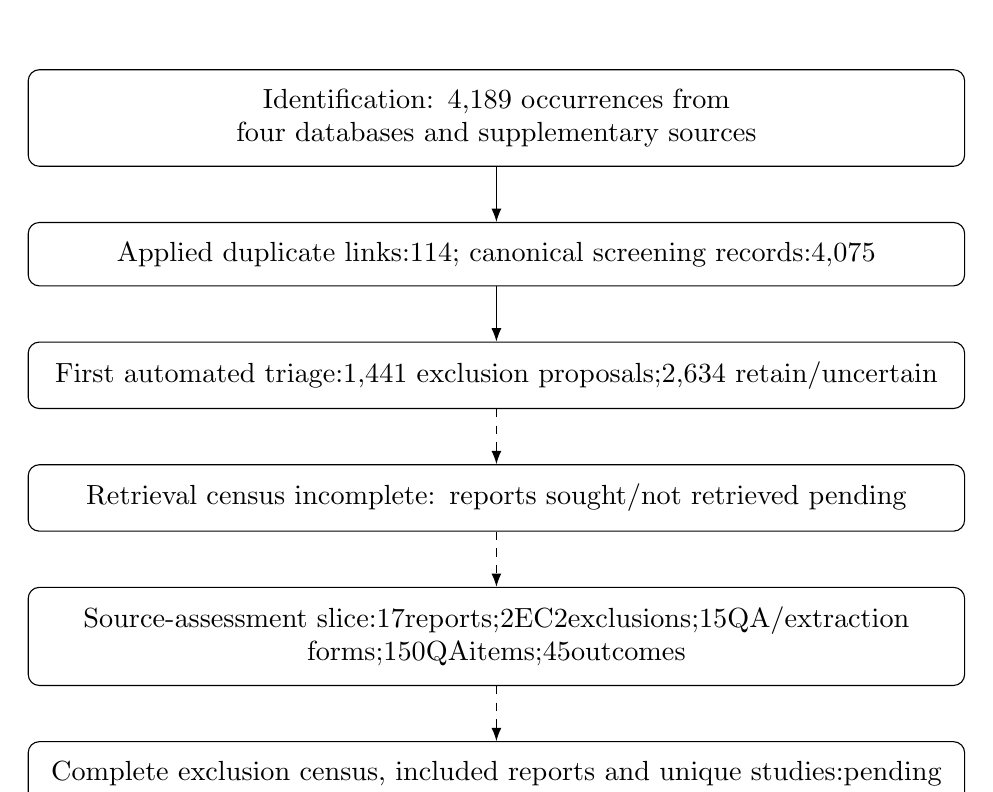
\begin{tikzpicture}[node distance=7mm,box/.style={draw,rounded corners,align=center,text width=11.4cm,inner sep=7pt},>=Latex]
\node[box](a){Identification: 4,189 occurrences from four databases and supplementary sources};
\node[box,below=of a](b){Applied duplicate links:114; canonical screening records:4,075};
\node[box,below=of b](c){First automated triage:1,441 exclusion proposals;2,634 retain/uncertain};
\node[box,below=of c](d){Retrieval census incomplete: reports sought/not retrieved pending};
\node[box,below=of d](e){Source-assessment slice:17reports;2EC2exclusions;15QA/extraction forms;150QAitems;45outcomes};
\node[box,below=of e](f){Complete exclusion census, included reports and unique studies:pending};
\draw[->](a)--(b);\draw[->](b)--(c);\draw[dashed,->](c)--(d);\draw[dashed,->](d)--(e);\draw[dashed,->](e)--(f);
\end{tikzpicture}\end{center}

{\small\begin{longtable}{>{\raggedright\arraybackslash}p{0.22\linewidth}>{\raggedright\arraybackslash}p{0.43\linewidth}>{\raggedright\arraybackslash}p{0.27\linewidth}}
\toprule
Report /\allowbreak{} decision & Source-based reason & Exact anchor\\\midrule
\endhead
GB-P016 TGS:\allowbreak{} Transparent GPU Sharing in Container Clouds for Deep Learning Workloads; EC2 & Training-focused GPU container sharing; evaluation concerns production/\allowbreak{}opportunistic training jobs. Discussion explicitly places inference optimization outside this paper; no separable inference-sharing result identified. & printed p69 abstract; evaluation pp75-80; p81 discussion; PDF pp2,8-14\\
GB-P017 HiveD:\allowbreak{} Sharing a GPU Cluster for Deep Learning with Guarantees; EC2 & GPU-cluster resource reservation and affinity for deep-learning training; evaluated queueing/\allowbreak{}completion-time behavior is not concurrent local inference serving. EC2 decisive; aggregate cluster scope is a secondary limitation. & printed p515 abstract; section6 evaluation pp521-525; PDF pp2,8-12\\
\bottomrule
\end{longtable}}


\section{Search, screening, duplicate and abstract logs}

The compact workbook carries 4,075 canonical screening rows and the 4,189-occurrence duplicate ledger. Screening rows contain database, year, DOI, first recommendation, reason, report/\allowbreak{}study links, full-text source/\allowbreak{}anchor and final status. Record IDs remain stable. The three merged canonical rows and original opinions are retained rather than deleted.


Whitespace/\allowbreak{}entity normalization was audited for all 4,189 abstract fields without publishing the full text or changing original exports.3,658 occurrences contain some abstract text and531 are blank. Normalization does not verify that a field is a complete abstract; snippets and truncation remain possible. The audit records character counts and source hashes rather than treating empty or incomplete text as a scientific finding.



\section{Quality assessment}

Group B uses ten 0-2 criteria. A reasoned N/\allowbreak{}A removes its maximum from the denominator. Below 60 percent is a sensitivity view, not an exclusion gate. All 15 assessed forms have ten item rows; none is converted to human-validated appraisal. The separate QA document supplies every rationale, anchor, assessor and remaining check.



{\small\begin{longtable}{>{\raggedright\arraybackslash}p{0.13\linewidth}>{\raggedright\arraybackslash}p{0.059\linewidth}>{\raggedright\arraybackslash}p{0.059\linewidth}>{\raggedright\arraybackslash}p{0.059\linewidth}>{\raggedright\arraybackslash}p{0.059\linewidth}>{\raggedright\arraybackslash}p{0.059\linewidth}>{\raggedright\arraybackslash}p{0.059\linewidth}>{\raggedright\arraybackslash}p{0.059\linewidth}>{\raggedright\arraybackslash}p{0.059\linewidth}>{\raggedright\arraybackslash}p{0.059\linewidth}>{\raggedright\arraybackslash}p{0.059\linewidth}>{\raggedright\arraybackslash}p{0.11\linewidth}}
\toprule
Report & Q1 & Q2 & Q3 & Q4 & Q5 & Q6 & Q7 & Q8 & Q9 & Q10 & Total\\\midrule
\endhead
GB-P001 & 2 & 2 & 1 & 1 & 1 & 2 & NA & 2 & 1 & 1 & 13/\allowbreak{}18\\
GB-P002 & 2 & 2 & 2 & 1 & 1 & 2 & 2 & 2 & 1 & 2 & 17/\allowbreak{}20\\
GB-P003 & 2 & 2 & 2 & 2 & 2 & 2 & 2 & 2 & 1 & 1 & 18/\allowbreak{}20\\
GB-P004 & 2 & 2 & 2 & 1 & 2 & 2 & 2 & 2 & 1 & 1 & 17/\allowbreak{}20\\
GB-P005 & 2 & 2 & 1 & 2 & 2 & 2 & 1 & 2 & 1 & 2 & 17/\allowbreak{}20\\
GB-P006 & 2 & 2 & 1 & 2 & 1 & 2 & 2 & 2 & NA & 2 & 16/\allowbreak{}18\\
GB-P007 & 2 & 2 & 2 & 2 & 1 & 2 & 2 & 2 & 2 & 2 & 19/\allowbreak{}20\\
GB-P008 & 2 & 2 & 1 & 2 & 2 & 2 & 1 & 2 & 2 & 1 & 17/\allowbreak{}20\\
GB-P009 & 2 & 2 & 1 & 1 & 1 & 2 & 2 & 2 & 1 & 2 & 16/\allowbreak{}20\\
GB-P010 & 2 & 2 & 1 & 2 & 1 & 2 & 2 & 2 & 1 & 2 & 17/\allowbreak{}20\\
GB-P011 & 2 & 2 & 1 & 1 & 1 & 2 & 1 & 2 & 1 & 1 & 14/\allowbreak{}20\\
GB-P012 & 2 & 2 & 1 & 1 & 1 & 2 & 2 & 2 & 1 & 1 & 15/\allowbreak{}20\\
GB-P013 & 2 & 2 & 1 & 1 & 1 & 2 & 1 & 2 & 1 & 2 & 15/\allowbreak{}20\\
GB-P014 & 2 & 2 & 1 & 2 & 1 & 2 & 2 & 2 & 1 & 1 & 16/\allowbreak{}20\\
GB-P015 & 2 & 2 & 1 & 1 & 2 & 2 & 2 & 2 & NA & 2 & 16/\allowbreak{}18\\
\bottomrule
\end{longtable}}

Provisional N/\allowbreak{}A judgments are VastPipe Q7, Paella Q9 and XSched Q9. Claim-specific applicability and the planned calibration remain open. Twenty legacy items have section/\allowbreak{}figure anchors without original printed-page mapping; additional section-only anchors remain visible in QA follow-up. Current first scores produce no below 60 percent forms, but incomplete eligibility/\allowbreak{}version checks prevent a strong robustness claim.



\section{Topic-specific extraction and study identities}

The compact summary below links each report to its mechanism, hardware and assessment status. The separate data-extraction document and workbook retain full study forms and all 45 outcome rows. Every reported metric has a value/\allowbreak{}unit, workload, comparator and anchor. Two additional calculations retain explicit formulas and inputs and remain separate from reported measurements. Unknown fields are not extracted; a not-reported label is scoped to the source section actually checked.


\subsection*{GB-P001 VastPipe}
\cite{GB-P001}

{\small\begin{longtable}{>{\raggedright\arraybackslash}p{0.22\linewidth}>{\raggedright\arraybackslash}p{0.7\linewidth}}
\toprule
Dimension & Source-linked extraction\\\midrule
\endhead
Identity & Li-Xian Ma and Le-Ping Wang and En Shao and Rong-Yu Cao and Guang-Ming Tan; 2025; Journal of Computer Science and Technology\\
Mechanism /\allowbreak{} GPU & tuned/\allowbreak{}default MPS comparison; prior source check only; NVIDIA A100 (existing source-check register)\\
Workload /\allowbreak{} conditions & VGG16+GoogLeNet (existing extraction rows); not extracted; not extracted\\
Comparator & No MPS /\allowbreak{} default MPS;exact quotas not extracted\\
Eligibility /\allowbreak{} source & provisionally\_\allowbreak{}eligible; pp457-459, sections6.7-6.9, Figs14-16\\
\bottomrule
\end{longtable}}

\subsection*{GB-P002 iGniter}
\cite{GB-P002}

{\small\begin{longtable}{>{\raggedright\arraybackslash}p{0.22\linewidth}>{\raggedright\arraybackslash}p{0.7\linewidth}}
\toprule
Dimension & Source-linked extraction\\\midrule
\endhead
Identity & Fei Xu and Jianian Xu and Jiabin Chen and Li Chen and Ruitao Shang and Zhi Zhou and Fangming Liu; 2023; IEEE Transactions on Parallel and Distributed Systems\\
Mechanism /\allowbreak{} GPU & MPS quota allocation and shadow process recovery;prior source check; NVIDIA V100 (existing source-check register)\\
Workload /\allowbreak{} conditions & AlexNet;ResNet50;VGG19;SSD; not extracted; batch3 for prediction check;W1 SLO10ms for recovery example\\
Comparator & Measured latency for prediction error;10ms SLO for recovery\\
Eligibility /\allowbreak{} source & provisionally\_\allowbreak{}eligible; pp820-824, sections4.2,5.1-5.4, Figs13-17\\
\bottomrule
\end{longtable}}

\subsection*{GB-P003 gpulets}
\cite{GB-P003}

{\small\begin{longtable}{>{\raggedright\arraybackslash}p{0.22\linewidth}>{\raggedright\arraybackslash}p{0.7\linewidth}}
\toprule
Dimension & Source-linked extraction\\\midrule
\endhead
Identity & Seungbeom Choi et al.; 2022; USENIX ATC22\\
Mechanism /\allowbreak{} GPU & MPS spatial partitions plus temporal batching; interference-aware gpulet scheduler; RTX2080Ti11GB; two GPUs/\allowbreak{}server, two servers; local pair measurements separated\\
Workload /\allowbreak{} conditions & GoogLeNet,LeNet,ResNet50,SSD-MobileNet,VGG16,MnasNet,MobileNetv2,DenseNet,BaseBERT (Table3); paired local inferences; system scenarios contain several models; Poisson inter-arrivals; model SLO5-202ms;99\% requests within SLO; median of3 runs (pp207-208)\\
Comparator & Solo latency for local Fig7; SBP and greedy best-fit for system scheduling\\
Eligibility /\allowbreak{} source & provisionally\_\allowbreak{}eligible; pp201-203 local mechanism/\allowbreak{}Fig7; p207 Tables2-3;pp208-209 system methodology\\
\bottomrule
\end{longtable}}

\subsection*{GB-P004 PipeSwitch}
\cite{GB-P004}

{\small\begin{longtable}{>{\raggedright\arraybackslash}p{0.22\linewidth}>{\raggedright\arraybackslash}p{0.7\linewidth}}
\toprule
Dimension & Source-linked extraction\\\midrule
\endhead
Identity & Zhihao Bai;Zhen Zhang;Yibo Zhu;Xin Jin; 2020; USENIX OSDI20\\
Mechanism /\allowbreak{} GPU & Temporal task switching; pipelined model transfer; active/\allowbreak{}standby workers and shared memory daemon; V10016GB PCIe3x16;T416GB PCIe3x8\\
Workload /\allowbreak{} conditions & ResNet152;Inception\_\allowbreak{}v3;Bert\_\allowbreak{}base; one training task preempted for one inference task; separable inference latency; training32;inference8;100-run averages;Fig6 reports minimum/\allowbreak{}maximum (p508)\\
Comparator & Ready model;stop-and-start;MPS using unified memory\\
Eligibility /\allowbreak{} source & provisionally\_\allowbreak{}eligible; p508 section6/\allowbreak{}6.1; p509 Tables3-4\\
\bottomrule
\end{longtable}}

\subsection*{GB-P005 REEF conference}
\cite{GB-P005}

{\small\begin{longtable}{>{\raggedright\arraybackslash}p{0.22\linewidth}>{\raggedright\arraybackslash}p{0.7\linewidth}}
\toprule
Dimension & Source-linked extraction\\\midrule
\endhead
Identity & Mingcong Han;Hanze Zhang;Rong Chen;Haibo Chen; 2022; USENIX OSDI22\\
Mechanism /\allowbreak{} GPU & Reset-based preemption;idempotent inference kernels;dynamic kernel padding;runtime/\allowbreak{}driver changes; AMD Radeon Instinct MI50:\allowbreak{}60CUs/\allowbreak{}16GB;REEF-N extension NVIDIA V100\\
Workload /\allowbreak{} conditions & ResNet152;DenseNet201;VGG19;Inceptionv3;DistilBERT; DISB A/\allowbreak{}B:\allowbreak{}1RT+1BE;C:\allowbreak{}1RT+5BE;D/\allowbreak{}E:\allowbreak{}5RT+5BE; Table2 RT100/\allowbreak{}220/\allowbreak{}100/\allowbreak{}20/\allowbreak{}20req/\allowbreak{}s;D uniform,E Poisson;BE closed-loop;batch not extracted\\
Comparator & RT-Only;SEQ;GPUStreams;separate wait-based preemption microbenchmark\\
Eligibility /\allowbreak{} source & eligible\_\allowbreak{}companion\_\allowbreak{}candidate; p548 section7.1 Table2;p549 section7.2 Fig11;section8 idempotence limitation\\
\bottomrule
\end{longtable}}

\subsection*{GB-P006 Paella:\allowbreak{} Low-latency Model Serving with Software-defined GPU Scheduling}
\cite{GB-P006}

{\small\begin{longtable}{>{\raggedright\arraybackslash}p{0.22\linewidth}>{\raggedright\arraybackslash}p{0.7\linewidth}}
\toprule
Dimension & Source-linked extraction\\\midrule
\endhead
Identity & Kelvin K.W. Ng; Henri Maxime Demoulin; Vincent Liu; 2023; SOSP 2023\\
Mechanism /\allowbreak{} GPU & Instrumented kernels; software scheduling; Tesla T4\\
Workload /\allowbreak{} conditions & Mixed inference; lognormal arrivals sigma1.5/\allowbreak{}2; Mixed inference; lognormal arrivals sigma1.5/\allowbreak{}2; not extracted\\
Comparator & CUDA-MS;Triton23.03;Paella ablations\\
Eligibility /\allowbreak{} source & provisionally\_\allowbreak{}eligible;study\_\allowbreak{}identity\_\allowbreak{}provisional; printed pp604-606; PDF pp10-12; sections7.1-7.3\\
\bottomrule
\end{longtable}}

\subsection*{GB-P007 Orion:\allowbreak{} Interference-aware, Fine-grained GPU Sharing for ML Applications}
\cite{GB-P007}

{\small\begin{longtable}{>{\raggedright\arraybackslash}p{0.22\linewidth}>{\raggedright\arraybackslash}p{0.7\linewidth}}
\toprule
Dimension & Source-linked extraction\\\midrule
\endhead
Identity & Foteini Strati; Xianzhe Ma; Ana Klimovic; 2024; EuroSys 2024\\
Mechanism /\allowbreak{} GPU & Interception; interference-aware kernel scheduling; V10016GB;A10040GB extension\\
Workload /\allowbreak{} conditions & High-priority plus best-effort inference;Poisson; High-priority plus best-effort inference;Poisson; not extracted\\
Comparator & Dedicated high-priority GPU;MPS;Streams;REEF-N policy\\
Eligibility /\allowbreak{} source & provisionally\_\allowbreak{}eligible;study\_\allowbreak{}identity\_\allowbreak{}provisional; printed pp1082-1087; PDF pp8-13; sections6-7\\
\bottomrule
\end{longtable}}

\subsection*{GB-P008 GSLICE:\allowbreak{} Controlled Spatial Sharing of GPUs for a Scalable Inference Platform}
\cite{GB-P008}

{\small\begin{longtable}{>{\raggedright\arraybackslash}p{0.22\linewidth}>{\raggedright\arraybackslash}p{0.7\linewidth}}
\toprule
Dimension & Source-linked extraction\\\midrule
\endhead
Identity & Aditya Dhakal; Sameer G Kulkarni; K.K. Ramakrishnan; 2020; SoCC 2020\\
Mechanism /\allowbreak{} GPU & MPS allocation; adaptive batching; One V10016GB\\
Workload /\allowbreak{} conditions & Concurrent inference functions;25ms target; Concurrent inference functions;25ms target; not extracted\\
Comparator & Default MPS;MPS+SLAB;TensorRT19.02\\
Eligibility /\allowbreak{} source & provisionally\_\allowbreak{}eligible;study\_\allowbreak{}identity\_\allowbreak{}provisional; printed pp499-501; PDF pp8-10; sections4.1-4.3\\
\bottomrule
\end{longtable}}

\subsection*{GB-P009 Serving DNNs like Clockwork:\allowbreak{} Performance Predictability from the Bottom Up}
\cite{GB-P009}

{\small\begin{longtable}{>{\raggedright\arraybackslash}p{0.22\linewidth}>{\raggedright\arraybackslash}p{0.7\linewidth}}
\toprule
Dimension & Source-linked extraction\\\midrule
\endhead
Identity & Arpan Gujarati; Reza Karimi; Safya Alzayat; Wei Hao; Antoine Kaufmann; Ymir Vigfusson; Jonathan Mace; 2020; USENIX OSDI 2020\\
Mechanism /\allowbreak{} GPU & Predictable temporal scheduling; One V10032GB in section6.1\\
Workload /\allowbreak{} conditions & 15 ResNet50 instances;16 closed-loop clients/\allowbreak{}model; 15 ResNet50 instances;16 closed-loop clients/\allowbreak{}model; not extracted\\
Comparator & Clipper;INFaaS (different EC2 hardware)\\
Eligibility /\allowbreak{} source & provisionally\_\allowbreak{}eligible;study\_\allowbreak{}identity\_\allowbreak{}provisional; printed pp451-452; author PDF pp9-10; section6.1/\allowbreak{}Fig5\\
\bottomrule
\end{longtable}}

\subsection*{GB-P010 Colocating ML Inference and Training with Fast GPU Memory Handover (SIRIUS)}
\cite{GB-P010}

{\small\begin{longtable}{>{\raggedright\arraybackslash}p{0.22\linewidth}>{\raggedright\arraybackslash}p{0.7\linewidth}}
\toprule
Dimension & Source-linked extraction\\\midrule
\endhead
Identity & Jiali Wang; Yankui Wang; Mingcong Han; Rong Chen; 2025; USENIX ATC2025, pp1657-1675\\
Mechanism /\allowbreak{} GPU & hybrid spatial sharing; CUDA VMM memory handover and dynamic SM masking; separate inference/\allowbreak{}training runtimes; single NVIDIA Tesla V100 16GB in section6.1; four-V100 host; separate section6.6 single A100 80GB LLM experiment\\
Workload /\allowbreak{} conditions & ResNet152 319MB; DenseNet169 84MB; EfficientNetV2-s86MB; EfficientViT-b2 109MB; DistilBERT254MB; DistilGPT2 317MB; Swin-T training; section6.6 Llama2-13B26GB with Qwen2-0.5B training; six inference models duplicated round-robin to56 instances; co-located Swin-T training, batch72; Light/\allowbreak{}Heavy/\allowbreak{}Burst/\allowbreak{}Skewed and compressed Azure Functions traces; 300s runs; SLO=4x standalone inference execution; Tidle5s, watermark1GB\\
Comparator & TaskSwitch implemented by authors, not vanilla PipeSwitch; SP-50/\allowbreak{}SP-75 static memory; UM+MPS; Infer-Only\\
Eligibility /\allowbreak{} source & provisionally\_\allowbreak{}eligible\_\allowbreak{}AI\_\allowbreak{}source\_\allowbreak{}assessment; printed pp1665-1666, section6/\allowbreak{}6.1, Table3, Figure10; PDF pp10-11 (includes cover)\\
\bottomrule
\end{longtable}}

\subsection*{GB-P011 ParvaGPU:\allowbreak{} Efficient Spatial GPU Sharing for Large-Scale DNN Inference in Cloud Environments}
\cite{GB-P011}

{\small\begin{longtable}{>{\raggedright\arraybackslash}p{0.22\linewidth}>{\raggedright\arraybackslash}p{0.7\linewidth}}
\toprule
Dimension & Source-linked extraction\\\midrule
\endhead
Identity & Munkyu Lee; Sihoon Seong; Minki Kang; Jihyuk Lee; Gap-Joo Na; In-Geol Chun; Dimitrios Nikolopoulos; Cheol-Ho Hong; 2024; SC2024 identity; extracted text is arXiv2409.14447v1\\
Mechanism /\allowbreak{} GPU & hybrid MIG+MPS; MPS processes within a MIG segment; profiler/\allowbreak{}configurator plus fleet allocator; A10080GB; Amazon p4de.24xlarge hosts with8 GPUs; extracted profiler point concerns one MIG segment\\
Workload /\allowbreak{} conditions & 11 DNN workloads overall; local extracted example InceptionV3; one to three homogeneous MPS processes within a MIG instance; other models can occupy separate segments; extracted example:\allowbreak{}1-GPC MIG instance; batch4;1/\allowbreak{}2/\allowbreak{}3 MPS processes; no tail quantile identified for local latency\\
Comparator & same InceptionV3/\allowbreak{}MIG/\allowbreak{}batch at1 MPS process versus2/\allowbreak{}3; fleet baselines not used for local effect\\
Eligibility /\allowbreak{} source & uncertain\_\allowbreak{}publication\_\allowbreak{}version;technical\_\allowbreak{}scope\_\allowbreak{}supported; author preprint PDF pp4-5 Figures3-4; p8 experimental environment\\
\bottomrule
\end{longtable}}

\subsection*{GB-P012 Torpor:\allowbreak{} GPU-Enabled Serverless Computing for Low-Latency, Resource-Efficient Inference}
\cite{GB-P012}

{\small\begin{longtable}{>{\raggedright\arraybackslash}p{0.22\linewidth}>{\raggedright\arraybackslash}p{0.7\linewidth}}
\toprule
Dimension & Source-linked extraction\\\midrule
\endhead
Identity & Minchen Yu; Ao Wang; Dong Chen; Haoxuan Yu; Xiaonan Luo; Zhuohao Li; Wei Wang; Ruichuan Chen; Dapeng Nie; Haoran Yang; Yu Ding; 2025; USENIX ATC2025 pp597-612\\
Mechanism /\allowbreak{} GPU & API redirection/\allowbreak{}remoting plus temporal request-level sharing and host/\allowbreak{}GPU model swapping; GPU runtime sharing mode; single V10032GB in local Figure8; evaluation worker has4 V10032GB GPUs\\
Workload /\allowbreak{} conditions & ResNet152 local sharing test;8 models in Table4 including DenseNet169/\allowbreak{}201,InceptionV3,EfficientNet,ResNet50/\allowbreak{}101/\allowbreak{}152,Bert-qa; multiple low-frequency ResNet152 functions share one GPU; sufficient functions to saturate device memory; 10-80 requests/\allowbreak{}minute/\allowbreak{}function; global defaultP98; CV deadline80ms and Bert-qa200ms\\
Comparator & Native early binding; local remoting microbenchmark also compares GVirtuS; cluster INFless-KA results kept separate\\
Eligibility /\allowbreak{} source & provisionally\_\allowbreak{}eligible\_\allowbreak{}AI\_\allowbreak{}source\_\allowbreak{}assessment; pp604-606 sections7.1-7.2, Table4, Figure8; PDF pp9-11\\
\bottomrule
\end{longtable}}

\subsection*{GB-P013 StreamBox:\allowbreak{} A Lightweight GPU SandBox for Serverless Inference Workflow}
\cite{GB-P013}

{\small\begin{longtable}{>{\raggedright\arraybackslash}p{0.22\linewidth}>{\raggedright\arraybackslash}p{0.7\linewidth}}
\toprule
Dimension & Source-linked extraction\\\midrule
\endhead
Identity & Hao Wu; Yue Yu; Junxiao Deng; Shadi Ibrahim; Song Wu; Hao Fan; Ziyue Cheng; Hai Jin; 2024; USENIX ATC2024 pp59-73\\
Mechanism /\allowbreak{} GPU & API forwarding into workflow-shared CUDA runtime/\allowbreak{}streams; PTB software spatial partitioning and fine-grained memory pool; V10016GB,80CUs; host has4 GPUs; single-GPU multi-user test in section9.4\\
Workload /\allowbreak{} conditions & Image Processing,Traffic,Social Media workflows:\allowbreak{} SSD300,FSRCNN,ResNet152/\allowbreak{}50/\allowbreak{}18,VGG16,AlexNet,LSTM,BERT; concurrent functions within workflow share runtime; separate3/\allowbreak{}6-user Traffic test on one GPU; Azure Functions7-day invocation trace; sporadic/\allowbreak{}periodic/\allowbreak{}bursty; Traffic SLO200ms; up to3 workflows/\allowbreak{}runtime contexts per GPU in evaluated setup\\
Comparator & INFless and Astraea with MPS; Stream-only; all warm-up/\allowbreak{}model-sharing/\allowbreak{}pipelined-loading settings disclosed in section9\\
Eligibility /\allowbreak{} source & provisionally\_\allowbreak{}eligible\_\allowbreak{}AI\_\allowbreak{}source\_\allowbreak{}assessment; pp67-70 sections9.1-9.4; Figures12-14,19; PDF pp10-13\\
\bottomrule
\end{longtable}}

\subsection*{GB-P014 Efficient Performance-Aware GPU Sharing with Compatibility and Isolation through Kernel Space Interception (KRYPTON)}
\cite{GB-P014}

{\small\begin{longtable}{>{\raggedright\arraybackslash}p{0.22\linewidth}>{\raggedright\arraybackslash}p{0.7\linewidth}}
\toprule
Dimension & Source-linked extraction\\\midrule
\endhead
Identity & Shulai Zhang; Ao Xu; Quan Chen; Han Zhao; Weihao Cui; Zhen Wang; Yan Li; Limin Xiao; Minyi Guo; 2025; USENIX ATC2025 pp1003-1019\\
Mechanism /\allowbreak{} GPU & kernel-command-buffer interception; feedback-controlled temporal quotas and MIG spatial orchestration; Linux loadable module; A10040GB for local quota/\allowbreak{}QoS tests; twoRTX4090 used for separate distributed-training test\\
Workload /\allowbreak{} conditions & local Transformer-XL inference batch8/\allowbreak{}16/\allowbreak{}32;ResNet50/\allowbreak{}MobileNetV2/\allowbreak{}BERT-Large also benchmarked; inference with co-running applications; separate training/\allowbreak{}rendering results not substituted; QoS:\allowbreak{}Poisson arrivals at half maximum throughput;50\%temporal allocation;5/\allowbreak{}10/\allowbreak{}20/\allowbreak{}40/\allowbreak{}80ms tokens; target original soloP99\\
Comparator & original soloP99 QoS target; fixed temporal quotas; adapted MIG baselines used separately for fleet packing\\
Eligibility /\allowbreak{} source & provisionally\_\allowbreak{}eligible\_\allowbreak{}AI\_\allowbreak{}source\_\allowbreak{}assessment; pp1011-1015 sections5.1,5.5-5.7,7; PDF pp10-14\\
\bottomrule
\end{longtable}}

\subsection*{GB-P015 XSched:\allowbreak{} Preemptive Scheduling for Diverse XPUs}
\cite{GB-P015}

{\small\begin{longtable}{>{\raggedright\arraybackslash}p{0.22\linewidth}>{\raggedright\arraybackslash}p{0.7\linewidth}}
\toprule
Dimension & Source-linked extraction\\\midrule
\endhead
Identity & Weihang Shen; Mingcong Han; Jialong Liu; Rong Chen; Haibo Chen; 2025; USENIX OSDI2025 pp671-692\\
Mechanism /\allowbreak{} GPU & temporal/\allowbreak{}preemptive runtime interposition via XQueue/\allowbreak{}XShim; hardware-specific preemption levels; single NVIDIA GV100 for extracted Triton/\allowbreak{}Paella case; NPU/\allowbreak{}ASIC/\allowbreak{}FPGA results outside extracted GPU outcomes\\
Workload /\allowbreak{} conditions & two Bert-large model clients for Triton; Paella mixed-model request workload for second case; one high-priority client at10requests/\allowbreak{}s;low-priority client continuous on sameGV100; Triton client rates as above;Paella workload lognormal sigma2.0;K-EDF K16; exact batch sizes not reported in extracted case3\\
Comparator & vanilla Triton;Triton priority setting;standalone high-priority execution;separate comparison to Paella\\
Eligibility /\allowbreak{} source & provisionally\_\allowbreak{}eligible\_\allowbreak{}AI\_\allowbreak{}source\_\allowbreak{}assessment; p683 section7.4 case3/\allowbreak{}Figure15; PDF p14\\
\bottomrule
\end{longtable}}


\section{Taxonomy and integration layers}
\begin{figure}[htbp]\centering
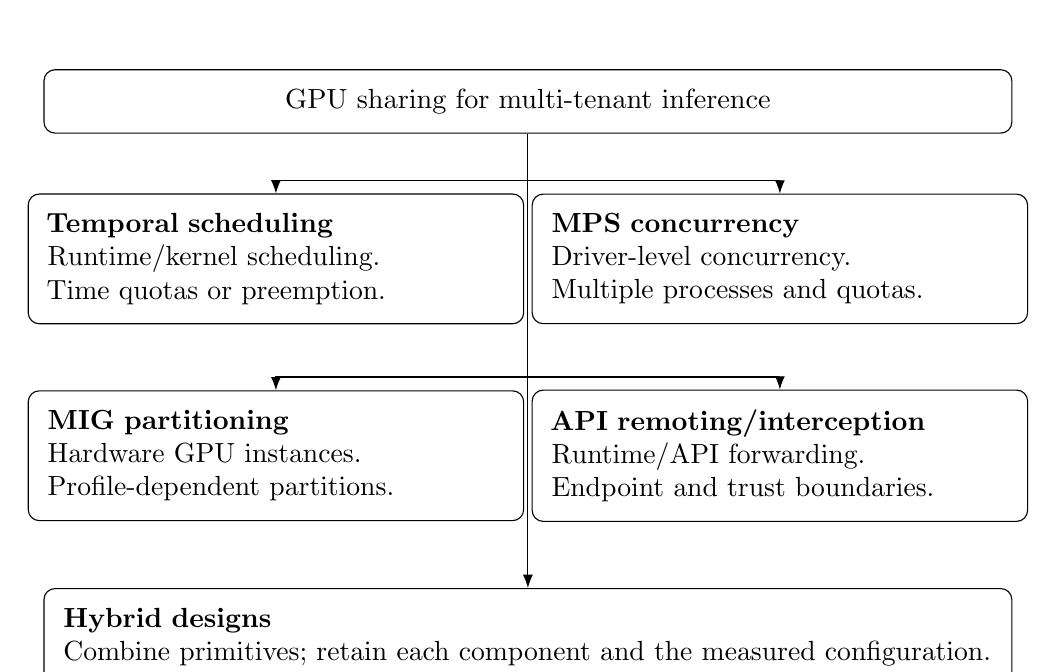
\begin{tikzpicture}[box/.style={draw,rounded corners,align=left,text width=5.8cm,inner sep=7pt},>=Latex]
\node[box,text width=11.8cm,align=center](root) at(0,0){GPU sharing for multi-tenant inference};
\node[box](t) at(-3.2,-2.0){\textbf{Temporal scheduling}\\Runtime/kernel scheduling.\\Time quotas or preemption.};
\node[box](m) at(3.2,-2.0){\textbf{MPS concurrency}\\Driver-level concurrency.\\Multiple processes and quotas.};
\node[box](g) at(-3.2,-4.5){\textbf{MIG partitioning}\\Hardware GPU instances.\\Profile-dependent partitions.};
\node[box](a) at(3.2,-4.5){\textbf{API remoting/interception}\\Runtime/API forwarding.\\Endpoint and trust boundaries.};
\node[box,text width=11.8cm](h) at(0,-6.8){\textbf{Hybrid designs}\\Combine primitives; retain each component and the measured configuration.};
\draw(root.south)--(0,-5.7);
\draw[->](0,-1.0)-|(t.north);\draw[->](0,-1.0)-|(m.north);
\draw[->](0,-3.5)-|(g.north);\draw[->](0,-3.5)-|(a.north);
\draw[->](0,-5.7)--(h.north);
\end{tikzpicture}
\caption{Group B mechanism taxonomy. Categories describe designs, not counts of finally included studies.}
\end{figure}


{\small\begin{longtable}{>{\raggedright\arraybackslash}p{0.24\linewidth}>{\raggedright\arraybackslash}p{0.68\linewidth}}
\toprule
Family & Assessed evidence /\allowbreak{} boundary\\\midrule
\endhead
Temporal/\allowbreak{}preemptive & PipeSwitch,REEF,Clockwork,Paella,Orion,XSched andTorpor contain different scheduling mechanisms; their priority, switching and batching costs are not interchangeable.\\
MPS concurrency & VastPipe,iGniter,gpulets andGSLICE use or compare local spatial concurrency; allocation and model mix change interference.\\
MIG /\allowbreak{} hybrid & KRYPTON integrates MIG with time quotas;ParvaGPU characterizes MIG+MPS but accessed version remains uncertain. No pooled hardware-isolation gain is inferred.\\
API interception/\allowbreak{}remoting & Torpor redirects APIs with model swapping;StreamBox forwards APIs into workflow runtimes;KRYPTON intercepts command buffers in kernel space. Those boundaries have different trust and integration costs.\\
Memory-sharing hybrids & SIRIUS uses VMM handover and SM masks across inference/\allowbreak{}training;StreamBox shares runtime/\allowbreak{}memory within a workflow.\\
\bottomrule
\end{longtable}}


\section{Comparative evidence}

Numerical comparisons are within-paper contrasts. They are not ranked across unmatched GPUs, models, batches, load generators, memory capacities or baselines. Each row retains a representative outcome; the complete 45-row register is separate.



{\small\begin{longtable}{>{\raggedright\arraybackslash}p{0.1\linewidth}>{\raggedright\arraybackslash}p{0.24\linewidth}>{\raggedright\arraybackslash}p{0.23\linewidth}>{\raggedright\arraybackslash}p{0.33\linewidth}}
\toprule
Report & Representative result & Comparator & Anchor /\allowbreak{} interpretation limit\\\midrule
\endhead
GB-P001 & Throughput ratio:\allowbreak{} 2.7 x & No MPS & pp457-458 Fig14 and accompanying prose; Batch/\allowbreak{}rate/\allowbreak{}quotas unresolved; not tail-latency evidence\\
GB-P002 & Prediction error range:\allowbreak{} 1.53-5.02 percent & Measured local latency & p822 section5.2 Fig13; Prediction accuracy, not utilization or latency speedup\\
GB-P003 & Distribution threshold:\allowbreak{}90\% of measured pairs:\allowbreak{} 17.66 percent overhead below threshold & Solo-running latency & p203 Fig7; Across-pair CDF, not request-p90/\allowbreak{}p99; no hostile-memory/\allowbreak{}fault test\\
GB-P004 & Additional end-to-end latency:\allowbreak{} 6.01 ms & Ready-model latency subtracted; MPS overhead307.02ms & p509 Table3; setup p508 section6; Mean100 runs; overhead, not total latency or p99; MPS uses unified-memory swapping\\
GB-P005 & Overall throughput ratio:\allowbreak{} 1.60 x & RT-Only dedicated GPU & p549 section7.2 Fig11 prose; setup p548 Table2; Includes RT and BE requests; RT-only reference dedicates GPU to RT tasks.\\
GB-P006 & ResNet18 p99 reduction factor:\allowbreak{} up to3 x & CUDA-MS & printed p604 section7.1/\allowbreak{}Fig12; PDF pp10-11; Author-reported approximate maximum; not uniform across loads\\
GB-P007 & Aggregate throughput ratio:\allowbreak{} up to7.3 x & Dedicated high-priority inference & printed p1086 section6.2.3/\allowbreak{}Fig12; PDF p12; Maximum; includes best-effort work\\
GB-P008 & GPU utilization efficacy GUE:\allowbreak{} 94.04 composite score & Default MPS GUE38.82 & printed p500 Table3; PDF p9; Not percent GPU utilization\\
GB-P009 & Clockwork goodput:\allowbreak{} approximately800 requests/\allowbreak{}second & INFaaS on nonidentical EC2 setup & printed p452 section6.1/\allowbreak{}Fig5; author PDF p10; Within-SLO successes; comparator qualitative; not total throughput\\
GB-P010 & Average P99 inference latency improvement factor, as reported:\allowbreak{} 12.6 x & TaskSwitch (authors' adapted temporal-switch baseline) & printed p1666, section6.1/\allowbreak{}Figure10 discussion; PDF p11; Author-reported average across tested workloads; not a uniform per-model speedup, and not a comparison to unmodified PipeSwitch.\\
GB-P011 & Reported throughput:\allowbreak{} 446 requests/\allowbreak{}s & same configuration with1 process (354requests/\allowbreak{}s) & author preprint PDF p5, sectionIII-B prose; Figure3 p4; One local configuration, not fleet savings. Source is arXivv1; final published version not verified.\\
GB-P012 & Reported single-GPU throughput factor:\allowbreak{} >10 x & Native early binding at same offered function rate & p606 section7.2; Figure8 p605; PDF pp10-11; Lower bound reported by authors, not an exact10x; function count varies to saturate memory. No fleet cost claim.\\
GB-P013 & Author-reported average throughput factor:\allowbreak{} 6.7 x & INFless with documented warm-up/\allowbreak{}pipelined loading/\allowbreak{}model sharing & p68 section9.1/\allowbreak{}Figure13; PDF p11; Aggregate within-paper result across tested workflows; not universal or a matched cross-paper speedup. Batch/\allowbreak{}concurrency optimizations contribute.\\
GB-P014 & Reported average QoS violation rate:\allowbreak{} 1.23 percent of requests & original soloP99 threshold (1\%baseline violations by definition) & p1014 section5.5/\allowbreak{}Figure17; PDF p13; Average across tested configurations; no claim that worst-case violation is1.23\%. Threshold-relative metric, not latency in milliseconds.\\
GB-P015 & Reported high-priorityP99 latency ratio:\allowbreak{} 1.07 x standalone & standalone high-priorityBert-large execution & p683 section7.4 case3/\allowbreak{}Figure15a; PDF p14; Triton+XSched;not a rawmillisecond value. NativeTriton ratio1.53x;noNPUresultincluded.\\
\bottomrule
\end{longtable}}


\section{Engineering trade-offs}


{\small\begin{longtable}{>{\raggedright\arraybackslash}p{0.26\linewidth}>{\raggedright\arraybackslash}p{0.66\linewidth}}
\toprule
Choice & Observed benefit /\allowbreak{} required sacrifice\\\midrule
\endhead
Tuned MPS & VastPipe throughput contrasts do not establish tail-latency or fault isolation; iGniter recovery traces retain transient SLO violation.\\
Preemptive priority & XSched high-priorityTritonP99 is1.07xstandalone versus1.53xnativeTriton, with a continuously busy background client; background throughput remains a separate objective.\\
Memory handover & SIRIUS improves local inference tails versus an adapted switch baseline while opportunistic training uses residual resources; training gains are not inference throughput.\\
Workflow runtime sharing & StreamBox eliminates runtime redundancy but cross-user concurrency can cause queuing and SLO violations; within-workflow address-space sharing limits isolation.\\
Remoting/\allowbreak{}model swapping & Torpor increases low-rate function density; heavy model transfers can increase latency sharply and add CPU/\allowbreak{}bandwidth demand.\\
Temporal quota granularity & KRYPTON token lengths trade scheduling overhead against wait time, differently for different batches.\\
MIG+MPS configuration & ParvaGPU preprint example changes throughput354to446requests/\allowbreak{}s while latency11to27ms; this is version-qualified local evidence, not a final included-study claim.\\
\bottomrule
\end{longtable}}


\section{Conflicting evidence and comparability}

Different results are not automatically contradictory. GSLICE reports a negative latency contrast against TensorRT in one configuration, while other outcomes evaluate different baselines and statistics. Torpor model swapping can hurt a heavy model even when function density improves. These within-paper differences support condition-aware choices rather than an averaged universal speedup.


The ParvaGPU local example illustrates a concrete tension:\allowbreak{} at1-GPC MIG size and batch4, moving from one to three MPS processes changes throughput354to446requests/\allowbreak{}s and latency11to27ms. The separately calculated increase is25.99percent throughput and2.4545xlatency, with explicit inputs retained. Latency percentile is unspecified and final publication equivalence is unresolved. These values are not pooled with P99/\allowbreak{}P98 request tails from other systems.


Cross-study comparisons remain qualitative where hardware, tenant mix, batching, load, runtime sharing or measurement intervals differ. No matched, controlled study-to-study contradiction or universal winning mechanism has been established by this checkpoint.



\section{Answers to the research questions}


{\small\begin{longtable}{>{\raggedright\arraybackslash}p{0.08\linewidth}>{\raggedright\arraybackslash}p{0.84\linewidth}}
\toprule
RQ & Evidence-based checkpoint answer\\\midrule
\endhead
RQ1 & The assessed slice covers temporal scheduling,MPS,API interception/\allowbreak{}remoting,memory-sharing hybrids and MIG-integrating designs. Prevalence across the literature cannot be inferred from the incomplete selected set.\\
RQ2 & The register distinguishes requests/\allowbreak{}s,throughput ratios,P99/\allowbreak{}P98,SLO-violation rate,API overhead and host/\allowbreak{}GPU memory. These are not interchangeable measures of utilization.\\
RQ3 & Batch,process count,arrival pattern,model size,runtime redundancy,hardware capability and memory/\allowbreak{}PCIe pressure alter outcomes. Local example settings accompany every metric.\\
RQ4 & Scheduling fairness and resource quotas have more direct evidence than general security/\allowbreak{}fault guarantees. Compiler transformation,kernel modules,model swapping and CPU-side API handling impose different costs.\\
RQ5 & Select a candidate mechanism by service priority and constraints, then validate it under the intended model mix and load. Final recommendation confidence is limited by incomplete eligibility,source versions and single-AI assessment.\\
\bottomrule
\end{longtable}}


\section{Conditional engineering recommendations}


{\small\begin{longtable}{>{\raggedright\arraybackslash}p{0.23\linewidth}>{\raggedright\arraybackslash}p{0.35\linewidth}>{\raggedright\arraybackslash}p{0.32\linewidth}}
\toprule
Scenario & Candidate /\allowbreak{} evidence & Cost and alternative\\\midrule
\endhead
Trusted multi-model inference with configurable quotas & Test MPS allocation approaches against native sharing on the targetGPU; VastPipe/\allowbreak{}iGniter/\allowbreak{}gpulets/\allowbreak{}GSLICE supply condition-specific leads. & Check tail latency and memory interference. Use stronger partitioning where trust boundaries require it; do not infer security from throughput.\\
Foreground request-tail priority & Test preemptive scheduling;XSchedTriton case andREEF/\allowbreak{}Orion/\allowbreak{}Paella offer different integration choices. & Account for hardware preemption support and background slowdown; use batching/\allowbreak{}dedication when isolation/\allowbreak{}integration demands dominate.\\
Workflow-local function density & TestStreamBox-style runtime/\allowbreak{}memory sharing where workflow functions share a trust boundary. & Requires compilation/\allowbreak{}profiling and controlled concurrency; separate runtimes/\allowbreak{}partitions suit stronger isolation requirements.\\
Many low-rate model functions & TestTorpor late binding against residentNative baselines under target model sizes. & Host memory,CPU andPCIe traffic increase; keep heavy/\allowbreak{}high-rate models resident when transfer cost dominates.\\
Mixed inference and opportunistic training & TestSIRIUS-type memory handover using separable inferenceSLO metrics. & Requires runtime integration and controlled memory reclamation;dedicate resources where interference risk is unacceptable.\\
MIG-aware deployments & TreatKRYPTON/\allowbreak{}ParvaGPU as design leads with different source/\allowbreak{}validation status. & Verify supportedprofiles,reconfiguration limits and finalsource;hardware partitions alone do not establish a measured end-to-endsecurity guarantee.\\
\bottomrule
\end{longtable}}


\section{Research gaps}

The checked set does not establish matched comparisons across all mechanisms on one common workload and hardware stack. Energy,security/\allowbreak{}fault tests,uncertainty intervals and software-version detail are uneven. The final report-to-study map,source-version checks and fullcandidate coverage remain incomplete. These gaps limit confidence before any deployment recommendation is generalized.



\section{Threats to validity and limitations}


{\small\begin{longtable}{>{\raggedright\arraybackslash}p{0.25\linewidth}>{\raggedright\arraybackslash}p{0.67\linewidth}}
\toprule
Threat & Handling /\allowbreak{} residual limitation\\\midrule
\endhead
Search reproducibility & Executed versus planned queries remain distinct; unresolved ACM/\allowbreak{}ScienceDirect totals and field/\allowbreak{}filter deviations are disclosed.\\
Selection bias & All records have initial automated triage, but 2,634 retain/\allowbreak{}uncertain records are not fully assessed. Accessible sources are a biased slice.\\
Reviewer judgment & AI-only continuation is disclosed. TwoAIopinions are not independent human validation; original scores/\allowbreak{}votes are preserved.\\
Source/\allowbreak{}version identity & ParvaGPUpreprint andREEFcompanion identity remain explicit. No inferred DOI substitution or automatic version merge.\\
Measurement interpretation & P99,P98,mean/\allowbreak{}unqualifiedlatency,model-pairpercentiles,training throughput and host-memory overhead remain separate.\\
Incomplete extraction & Not-extracted fields and section-scoped absence reporting remain visible; missing values are not zeros.\\
Final accounting & The final included-study count and final PRISMA stages remain pending; 15 forms do not meet the final-study target by themselves.\\
\bottomrule
\end{longtable}}

The submitted Task 1 protocol is byte-for-byte preserved. The current workbook, PDFs and supporting CSV files describe the same current register checkpoint. This is an updated evidence report with explicit unfinished review work, not a claim that every candidate has completed full-text eligibility.


\clearpage\bibliographystyle{ieeetr}\bibliography{references}\end{document}